\chapter{Nested Class Modularity in Squeak}
\label{sec:concept}
In this chapter, we describe the main concept of this work: classes as class members. Similar concepts are part of programming languages like Java, Ruby, Python, and Newspeak. Our concept follows closely the Newspeak notion of nested classes, but without making invasive changes to the Smalltalk programming language or the underlying virtual machine.

\section{Nested Classes}
In Smalltalk, every object is an instance of a class, defining the object's instance variables and the messages it understands. Consequently, a class is also an instance of its so-called meta class. Every meta class is an instance of \texttt{Metaclass} (Figure~\ref{fig:impl_squeak_meta}). In the remainder of this work, we denote the meta class of a class \texttt{C} by \texttt{C class}. Every Smalltalk image has a \texttt{globals} dictionary\footnote{Squeak also supports \emph{environments}, effectively making it possible to compile methods in the context of another \texttt{globals} dictionary. See Section~\ref{sec:rel_sq_env} for more details.}, mapping symbols to class objects (or other objects), so that references to classes can be resolved at compile time. This implies that all references to classes are early bound.

\msname extends the Smalltalk class organization as follows: in addition to regular methods, we introduce the concept of \emph{class generator methods}. Such a method generates a class and is associated with a set $I$ of instance methods and a set $C$ of class methods. Whenever the method is invoked, the system first executes the method body, then adds $I$ to the resulting class and $C$ to the resulting meta class, and finally returns the resulting class. For performance reasons, \msname also caches the result, meaning that a class is only generated once\footnote{Parameterized classes are an exception.}.

\paragraph{Details}
Class generator methods are only allowed as class-side methods. Class generators as instance-side methods seem to provide neglectable benefits and make the implementation of our system more complicated. We discuss instance-side class generator methods in more detail in the Section~\ref{sec:future_inst_side}.

A class generated by a class generator method is anonymous: it is not listed in the \texttt{globals} dictionary and can only be referenced using message sends to its enclosing class\footnote{It can also be referenced by sending the \texttt{class} message to one of its instances}. Consequently, its name is a concatenation of all class names on the path from the top-level class to the class in question.


\paragraph{Notation and Example}
\begin{wrapfigure}{l}{0.5\textwidth}
	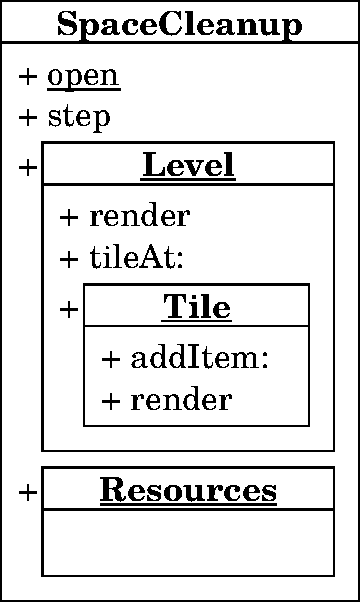
\includegraphics[scale=0.75]{nested_notation.pdf}
	\centering
	\caption[Example: Nested classes]{Example: nested classes. A class can have class-side member classes.}
	\label{fig:concept_nested_notation}
\end{wrapfigure}

Figure~\ref{fig:concept_nested_notation} shows an example of nested classes in \msname. \texttt{SpaceCleanup} is a top-level class, i.e., it is part of the \texttt{globals} dictionary and known everywhere in the system; it can be referenced by just writing the identifier \texttt{SpaceCleanup}. It has one instance method \texttt{step} and two class methods \texttt{open} and \texttt{Level}. In accordance with UML notation, class-side method selectors are underlined. 

\texttt{SpaceCleanup class>>Level} is a class generator method that is associated with a set of instance methods $\{\mbox{\texttt{render}, \texttt{tileAt:}}\}$ and a set of class methods $\{\mbox{\texttt{Tile}}\}$. The name of the class it generates is \texttt{SpaceCleanup Level}, which is in that case also a valid Smalltalk code expression that evaluates to the generated class. \texttt{SpaceCleanup class>>Level class>>Tile} is a class generator method that generates \texttt{SpaceCleanup Level Tile}. Note, that we use the \texttt{>>} notation to not only reference methods but also the classes they generate, in case they are class generator methods.

Top-level classes are called \emph{modules}. All other classes are called \emph{nested classes}. The class in which another class is nested is called the \emph{enclosing class}.

%\begin{figure}[!htp]
%	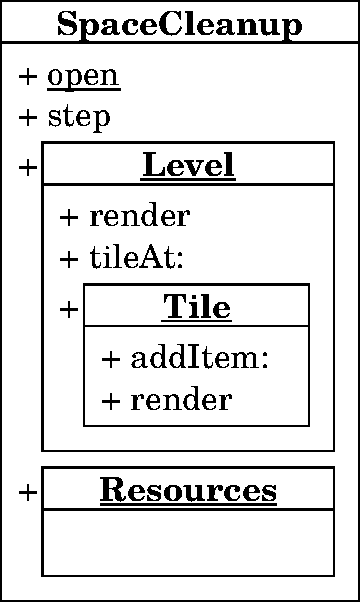
\includegraphics[scale=0.5]{nested_notation.pdf}
%	\centering
%	\caption{Nested Classes Example}
%	\label{fig:concept_nested_notation}
%\end{figure}

\section{Accessing the Lexical Scope}
Within a method, it might be necessary to access the lexical scope, in order to send messages to enclosing classes. For example, a method might want to reference a class defined in an enclosing class (e.g., \texttt{SpaceCleanup Resources} in \texttt{SpaceCleanup class>>Level class>>Tile>>render}). For this reason, \msname introduces new keywords, in addition to \texttt{self} and \texttt{super}, which are already present in every Smalltalk dialect. This is a point where we extended the programming language. Figure~\ref{fig:concept_keywords} gives an overview of all method lookup-related keywords in the system.

\begin{figure}[!htp]
	\centering
	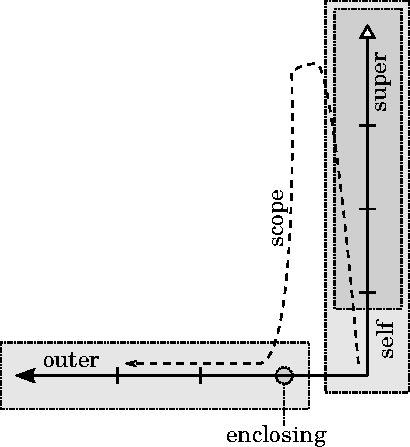
\includegraphics[scale=1]{lookup_keywords.pdf}
	\caption[Keywords for superclass and lexical scope access]{Keywords for superclass and lexical scope access. The lookup starts at \texttt{self}, and continues with the lexical scope.}
	\label{fig:concept_keywords}
\end{figure}

\subsection{\texttt{self} Keyword}
This keyword is used make a message send within an object. The receiver is the same object as the sender and the lookup starts at the (polymorphic) class of the receiver. If that class does not provide a corresponding method, the lookup continues in the superclass hierarchy. If no class in the superclass hierarchy has a corresponding method, a \texttt{MethodNotUnderstood} error is raised.

\begin{wrapfigure}{l}{0.5\textwidth}
	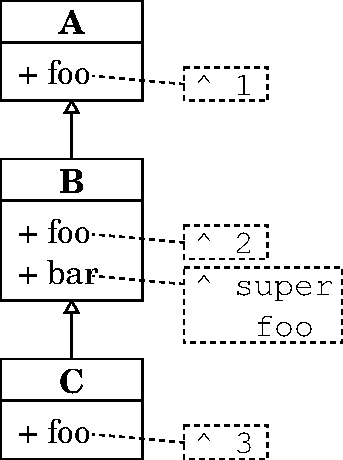
\includegraphics[scale=0.75]{super_binding.pdf}
	\centering
	\caption[Example: Binding of \texttt{super}]{Example: Binding of \texttt{super}. The method lookup starts at the superclass of the calling method's class.}
	\label{fig:concept_super_binding}
\end{wrapfigure}

\subsection{\texttt{super} Keyword}
This keyword is also used to make a message send within an object. Again, the receiver is the same object as the sender, but the lookup starts at the superclass of the sender's method class. Note, that \texttt{super} is bound to the superclass of the method class, not the superclass of the receiver's class. For example, in Figure~\ref{fig:concept_super_binding}, \texttt{Monster new defaultImage} returns \texttt{Resources errorPic}, because, in \texttt{MovingItem>>defaultImage}, \texttt{super} is bound to \texttt{Item}, even though the receiver \texttt{Monster new} is an instance of \texttt{Monster}.

\subsection{\texttt{enclosing} Keyword}
This keyword is an implementation artifact. It can be used for meta programming purposes, but should be avoided in general. It is used to make a message send to the class that contains the current class. Consider, for example, that we want to send a message \texttt{levelBackground} to class \texttt{SpaceCleanup Resources} within \texttt{SpaceCleanup class>>Level>>render} in Figure~\ref{fig:concept_nested_notation}. Either one of the following two statements works in this case\footnote{The enclosing class of an object that is not a class is its class' enclosing class.}.

\begin{itemize}
	\item \texttt{SpaceCleanup Resources levelBackground.}
	\item \texttt{enclosing Resources levelBackground.}
\end{itemize}

\texttt{enclosing} is a keyword that evaluates to the method owner's enclosing class upon method compilation. Note, that \texttt{enclosing} is bound to the method's lexical scope, not the receiver class' lexical scope.

Figure~\ref{fig:concept_lexical_thisouter} illustrates how \texttt{enclosing} is bound. In \texttt{SpaceCleanup class>>Item class>>player}, \texttt{enclosing} is bound to \texttt{SpaceCleanup}. In contrast, \texttt{UberSpaceClean\-up class>>Item class>>evilMonster} binds \texttt{enclosing} to \texttt{UberSpaceCleanup}. Consequently, \texttt{SpaceCleanup Item monster} calls \texttt{SpaceCleanup Resources monster} and so does \texttt{UberSpaceCleanup Item monster}, even though the receiver of \texttt{monster} is \texttt{UberSpaceCleanup Item} and not \texttt{SpaceCleanup Item} in the latter case. Note, that \texttt{UberSpaceCleanup Item evilMonster} calls the method in \texttt{UberSpaceCleanup Resources}, because \texttt{evilMonster}'s lexically enclosing class is \texttt{UberSpaceCleanup}.

\begin{figure}[!htp]
	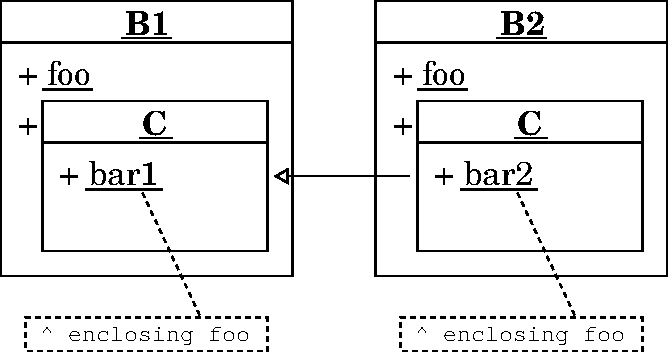
\includegraphics[scale=0.75]{nested_lexical1.pdf}
	\centering
	\caption[Example: Binding of \texttt{enclosing}]{Example: Binding of \texttt{enclosing}. The keyword is bound to enclosing class of the class where the method containing the keyword is contained.}
	\label{fig:concept_lexical_thisouter}
\end{figure}

Note, that \texttt{enclosing} can be used for meta programming purposes; however, it should be avoided in general, because it can lead to fragile code that makes too many assumptions about the structure of the class nesting. A later refactoring could then lead to broken code. Probably for the same reason, Smalltalk does not have a \texttt{super} keyword that does the lookup only in the superclass\footnote{However, there is a method \texttt{Class>>superclass}.} (single-level super). \msname provides a \texttt{scope} keyword that should be used instead.

\subsection{\texttt{enclosing} Method}
In addition to \texttt{enclosing}, every class in the system has a method \texttt{enclosing} that returns the enclosing class (\emph{owner}) of the receiver, making it possible to send messages to enclosing classes which are more than one level away. If, for example, in Figure~\ref{fig:concept_nested_notation}, \texttt{SpaceCleanup class>>Level class>>Tile>>render} wants to send the message \texttt{tileBackground} to \texttt{SpaceCleanup Resources}, either one of the following two statements works.

\begin{itemize}
	\item \texttt{SpaceCleanup Resources tileBackground.}
	\item \texttt{enclosing enclosing Resources tileBackground.}
\end{itemize}

Again, the method \texttt{enclosing} should be avoided in general, but is useful to implement parts of our system with code written in the system itself and for meta programming purposes. The statement \texttt{enclosing enclosing} would be somewhat similar to a \texttt{super super} statement. Arguably, this can result in verbose and complicated code, and is at the very least questionable with regards to the law of demeter. Note, that, in contrast to the \texttt{outer} keyword, the message send of \texttt{enclosing} to \texttt{enclosing} is no longer bound to the lexical scope of the method.

\subsection{\texttt{outer} Keyword}
\label{sec:concept_outer}
This keyword is used to make a message sends to classes in the lexical scope. Whenever a message is sent to \texttt{outer}, the message is first interpreted as a send to \texttt{enclosing}. If that message send fails, the message is sent to the second-level enclosing class in the current lexical scope. Eventually, the message is sent to a top-level class, if no other class understands the message. If even that message send is not understood, the selector is looked up in the \texttt{globals} dictionary. If the selector is absent, a \texttt{MessageNotUnderstood} error is raised.

\texttt{outer} is similar to \texttt{super}, with the difference that \texttt{outer} does a horizontal lookup (lexical scope) and \texttt{super} does a vertical lookup (superclass chain). Note, that messages sent to \texttt{outer} are sent to an object different from \texttt{self}.

\paragraph{Example}
Figure~\ref{fig:concept_outer_1} illustrates how message sends to \texttt{outer} are looked up. Consider, for example, that the method \texttt{render} in \texttt{SpaceCleanup class>>Level class>>Tile} calls \texttt{outer Resources tileBackground}. The method \texttt{SpaceCleanup class>>Level class>>Tile>>render} as well as the method \texttt{UberSpaceCleanup class>> Level class>>Tile>>render} call \texttt{SpaceCleanup Resources tileBackground} in this case, because \texttt{outer} is bound to the lexical scope of the method.

Figure~\ref{fig:concept_outer_2} shows why it is important that \texttt{outer} is bound to the lexical scope. In this example, \texttt{SpaceCleanupTest DummyLevel} is a subclass of \texttt{SpaceCleanup Level}. If the \texttt{outer} lookup simply traversed the chain of enclosing classes of the (late bound) receiver class, i.e., first lookup in \texttt{self enclosing}, then \texttt{self enclosing enclosing}, etc., the message send of \texttt{Resources} would fail in \texttt{SpaceCleanupTest class>>DummyLevel class>>Tile>>render}, because \texttt{SpaceCleanupTest} does not understand \texttt{Resources}.

\begin{figure}[!htp]
\begin{subfigure}[b]{\textwidth}
	\centering
	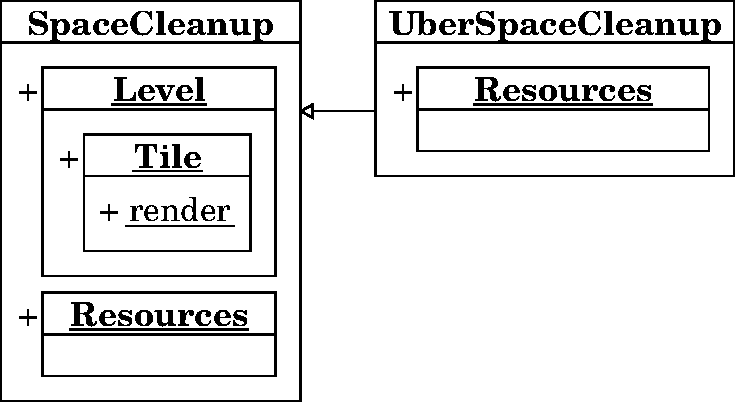
\includegraphics[scale=0.75]{outer_keyword.pdf}
	\caption{Subclassed top-level class}
	\label{fig:concept_outer_1}
\end{subfigure}

\vspace{15pt}

\begin{subfigure}[b]{\textwidth}
	\centering
	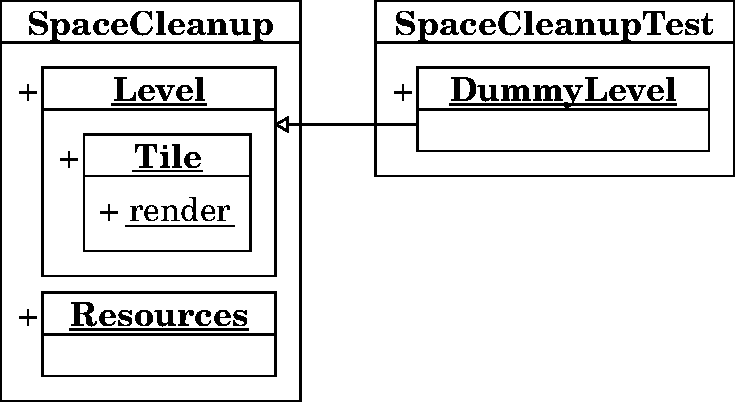
\includegraphics[scale=0.75]{outer_keyword_2.pdf}
	\caption{Subclassed nested class with different enclosing class}
	\label{fig:concept_outer_2}
\end{subfigure}

\caption[Example: \texttt{outer} keyword]{Example: \texttt{outer} keyword. Message sends to \texttt{outer} are looked up with respect to the lexical scope of the method, instead of following the chain of enclosing classes (owner hierarchy).}
\end{figure}

%The method \texttt{enclosing} can be used to traverse the the lexical scope of a class. Arbitrarily many \texttt{enclosing} sends can be chained, as long as the respective receiver still has an enclosing class and is, therefore, not a top-level class. Arguably, this can result in verbose and complicated code, and is at the very least questionable with regards to the law of demeter.

%In addition to \texttt{enclosing}, \msname provides the \texttt{outer} keyword, bound to the method's lexical scope. 

% If that message send fails, the message is sent to \texttt{enclosing enclosing}, and, eventually, to the top-level class, if no other class in the lexical scope understands the message. 

\subsection{\texttt{scope} Keyword}
This keyword combines \texttt{super} and \texttt{outer}: a message sent to \texttt{scope} is first treated as a \texttt{self} send. If the message is not understood, it is treated as an \texttt{outer} send.

\msname essentially first looks up the methods in \texttt{self}, then in the superclass hierarchy, and then in the lexical scope. This is how the method lookup in Java works, also known as \emph{comb semantics}~\cite{bracha2007interaction}. Newspeak uses a different lookup: it first looks for a method in the receiver's class, then in the lexical scope, and finally in superclass hierarchy~\cite{bracha:modules_as_objects}.

%The statement \texttt{enclosing enclosing m1} in the previous example can also be written as \texttt{scope m1}. If the method \texttt{m1} would now be moved to its enclosing class (if it had one), the lookup would still succeed. However, \texttt{scope} exposes the risk of accidentially capturing method names in superclasses or the lexical chain.

\subsection{Implicit \texttt{scope} Receiver}
\label{sec:con_implz_recv}
In \msname, references to globals are in fact message sends with \texttt{scope} as implicit receiver. This should make it easier for Smalltalk programmers to write code in \msname, even if they do not know about \texttt{enclosing} and \texttt{scope}. It also makes the code less verbose and easier to read.

Whenever code references an identifier that is not a temporary variable, not an instance variable, and not a \emph{special} object/keyword\footnote{\texttt{self}, \texttt{super}, \texttt{thisContext}, \texttt{scope}, \texttt{outer}, \texttt{enclosing}}, the compiler replaces that identifier with a message send to \texttt{scope}.

Consider, for example, that we want to reference class \texttt{SpaceCleanup Resources} within \texttt{SpaceCleanup class>>Level class>>Tile>>render} in Figure~\ref{fig:concept_nested_notation}. Either one of the following two statements works in this case.

\begin{itemize}
	\item \texttt{SpaceCleanup Resources.}
	\item \texttt{enclosing enclosing Resources.}
	\item \texttt{outer Resources.}
	\item \texttt{scope Resources.}
	\item \texttt{Resources.}
\end{itemize}

In this example, we used the implicit \texttt{scope} receiver for class lookup, which is in our opinion the most useful case. However, any unary method in \texttt{self}, the lexical scope, or the superclass hierarchy can be looked up this way. We think that this is bad practice and should be used only for class generator methods\footnote{It might be forbidden in future versions of \msname.}. It is allowed in Newspeak and other programming languages like Java, but these programming languages support implicit receivers by default. In Smalltalk, this is not the case and looks \emph{unfamiliar}. Classes are, however, just globals in Smalltalk and we emulate the notation for accessing them with an implicit \texttt{scope} receiver in \msname. 

Note, that only unary messages can have an implicit \texttt{scope} receiver, since we would have to change the Smalltalk syntax, otherwise.

\section{Parameterized Classes}
\label{sec:conz_param_cls}
In \msname, classes are accessed using message sends. Since messages can have parameters, it seems natural to have parameterized class accessor methods, and, therefore, parameterized classes. All examples shown in the previous sections use unparameterized classes, i.e., class generator methods are always unary. Class generator methods can, however, also have binary selectors or selectors with a higher arity. For memory conservation reasons, these classes are then no longer cached.

Parameterized classes can be used to make modules externally configurable or to implement mixins. We will present some conrete use cases in Section~\ref{sec:usecases}.

The arguments passed to a parameterized class generator method are considered when a message is sent to \texttt{enclosing}. At first, the system tries to send the message to the enclosing class. If that fails, \msname checks if the selector corresponds to one of the parameter names in the enclosing class' class generator method.

\begin{wrapfigure}{l}{0.5\textwidth}
	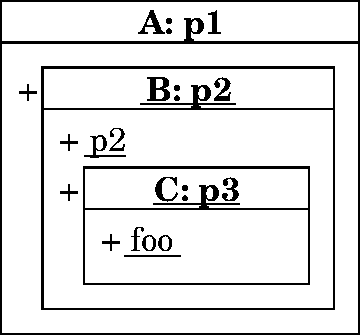
\includegraphics[scale=0.75]{nested_notation_params.pdf}
	\centering
	\caption[Example: Parameterized classes]{Example: Parameterized classes. A class can have parameters accessible with message sends to \texttt{enclosing}.}
	\label{fig:concept_param_classes}
\end{wrapfigure}

Consider, for example, that method \texttt{A: class>>B: class>>C: class>>foo} (see Figure~\ref{fig:concept_param_classes}) contains the following statements.
\begin{itemize}
	\item \texttt{scope p3}: method lookup succeeds in \texttt{A: class>>B: class>>C:} and returns the class parameter \texttt{p3}.
	\item \texttt{scope p2}: method lookup succeeds in \texttt{A: class>>B:} and calls the method \texttt{p2}, which shadows the class parameter \texttt{p2}.
	\item \texttt{scope p1}: method lookup succeeds in \texttt{A:} and returns the class parameter \texttt{p1}.
\end{itemize}

\section{Inheriting Nested Classes}
\label{sec:concept_inh_nested_cl}
Nested classes are accessed using methods returning the generated class. They are similar to class instance variables in a sense that nested classes belong to the enclosing class object. Therefore, a subclass of the enclosing class has its own nested class, i.e., the nested classes might have the same methods and variables declared, but they are different objects. Nested classes can be overridden in subclasses of enclosing classes, just as regular methods can be overridden. The following paragraphs give an overview of how a subclass of an enclosing class can customize the nested class.

\paragraph{Override with Nested Class}
A subclass of an enclosing class can define a new nested class. The programmer simply adds a new class generator method with the same selector to the subclass. The superclass will keep using the old nested class, whereas the subclass will use the new one, because the method lookup ends in the subclass when the corresponding class accessor method is found. The new nested class will only have the methods defined for the subclass' nested class and not inherit or copy any methods from the superclass' nested class.

\paragraph{Override with Regular Method}
A subclass of an enclosing class can replace (override) a nested class with a regular method. The programmer simply adds a new method which is not a class generator method to the subclass.

\paragraph{Extend Inherited Nested Class without Subclassing}
A subclass can extend the inherited nested class, i.e., the nested class in the subclass will have the same superclass as the nested class in the superclass. However, the nested class in the subclass will have all methods defined for the nested class in the superclass and additionally all methods defined for the nested class in the subclass. Duplicate methods will be replaced, similarly to extension methods in Squeak.

\begin{figure}[!htp]
\begin{subfigure}[b]{\textwidth}
	\centering
	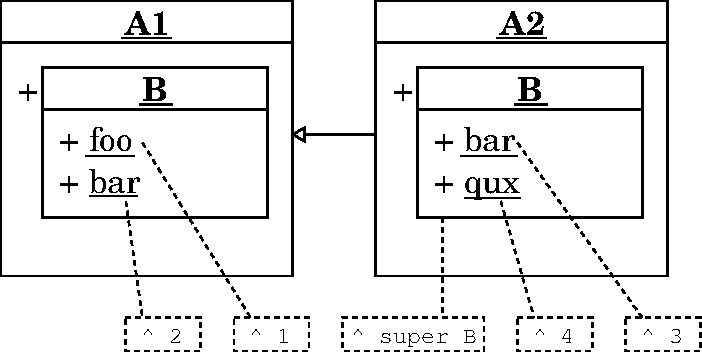
\includegraphics[scale=0.75]{nested_super_1.pdf}
	\caption{Extending inherited nested classing}
	\label{fig:impl:extend_inherited_class}
\end{subfigure}

\vspace{15pt}

\begin{subfigure}[b]{\textwidth}
	\centering
	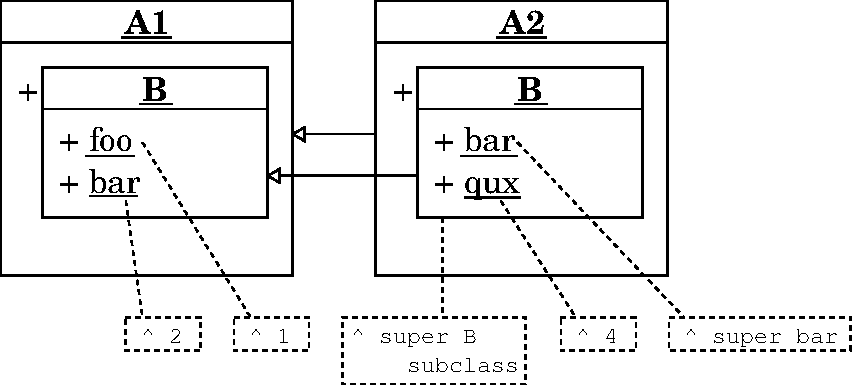
\includegraphics[scale=0.75]{nested_super_2.pdf}
	\caption{Subclassing inherited nested classing}
	\label{fig:impl:subclass_inherited_class}
\end{subfigure}

\caption[Example: Extending/subclassing nested classes]{Example: Extending and subclassing nested classes. Subclassing inherited nested classes leads to parallel class hierarchies.}
\end{figure}

Figure~\ref{fig:impl:extend_inherited_class} shows an example of a nested class extension. Class \texttt{A2} is a subclass of \texttt{A1}, which defines a nested class \texttt{B}. Therefore, both classes \texttt{A1} and \texttt{A2} have a nested class \texttt{B}. \texttt{A2} extends \texttt{B} by perfoming a super call. The following list gives an overview of how the classes \texttt{B} behave.

\begin{itemize}
	\item \texttt{A1 B foo}: returns 1.
	\item \texttt{A1 B bar}: returns 2.
	\item \texttt{A1 B qux}: raises \texttt{MessageNotUnderstood}, because \texttt{qux} is not defined on \texttt{A1 B}.
	\item \texttt{A2 B foo}: returns 1, because \texttt{A2 B} has all methods defined for \texttt{A1 B}.
	\item \texttt{A2 B bar}: returns 3, because that method was replaced in \texttt{A2 B}.
	\item \texttt{A2 B qux}: returns 4.
\end{itemize}

Note, that \texttt{A1 B} and \texttt{A2 B} have the same superclass, but are different class objects. \texttt{A2 B} is \emph{not} a subclass of \texttt{A1 B}. When \texttt{A2 B} is invoked for the first time, \msname first generates the class \texttt{A1 B} (because of the \texttt{super} call) and caches it for \texttt{A2 B}\footnote{Caches are receiver-specific.}. That class is then \emph{reinitialized} according to \texttt{A2 B} (without making a subclass), i.e., all methods defined for \texttt{A2 B} are added. A subsequent call to \texttt{A1 B} will not return the previous generated and extended class for \texttt{A2}, because the class cache works on a per-receiver basis.

Also note, that if we actually wanted to extend \texttt{A1 B} and alias it as \texttt{A2 B}, which is technically similar to an extension method in Smalltalk (see Section~\ref{sec:usecases_ext_meth}), then \texttt{A2 B} should be defined as \texttt{\^{} A1 B}, because the receiver of the message \texttt{B} will then be \texttt{A1} instead of \texttt{A2}. 

At the moment, there is no way to add additional instance variables or class variables to an extended nested class, because the class definition (containing the definition of variables) is done in the \texttt{super} call. 

\paragraph{Subclass Inherited Nested Class}
A subclass can subclass the inherited nested class, i.e., the nested class in the subclass is a subclass of the nested class in the superclass. Effectively, this results in a parallel class hierarchy. The nested subclass can override methods and use \texttt{super} to call methods in the nested superclass.

Figure~\ref{fig:impl:subclass_inherited_class} shows an example for subclassing a nested class, which is similar to Figure~\ref{fig:impl:extend_inherited_class}. Note, that \texttt{A2 B} is now a subclass of \texttt{A1 B} and \texttt{super} calls in \texttt{A2 B} now start their lookup in \texttt{A1 B}. The new subclass \texttt{A2 B} behaves like the class in the previous example, except for \texttt{A2 B bar}. That statement returns 2, because the \texttt{super} call invokes \texttt{A1 class>>B class>>foo}.

